\documentclass{article}

\usepackage[utf8]{inputenc}
\usepackage[T1]{fontenc}
\usepackage[ngerman]{babel}
\usepackage{graphicx}
\usepackage{float}
\usepackage{amsmath}
\usepackage{amssymb}
\usepackage{booktabs}
\usepackage{multirow}
\usepackage{siunitx}
\usepackage{csquotes}

\sisetup{
    locale = DE,
    separate-uncertainty = true,
    per-mode = symbol
}

\usepackage[
    backend=biber,
    style=numeric,
]{biblatex}

\addbibresource{quellen.bib}

\title{Photo- und Elektrolumineszenz in Halbleitern\\
Fortgeschrittenenpraktikum}
\author{Fynn Kanja 3780065\\
Valentino D'Agosto 3763229\\
Gruppe O43}
\date{Experiment durchgeführt am: 9. Juni 2026}

\setlength{\parindent}{0pt}
\setlength{\parskip}{1em}
\emergencystretch=2em

\begin{document}

\begin{figure}
    \centering
    
\includegraphics[width=0.75\linewidth]{uni_logo.png}
\end{figure}

\maketitle

\begin{abstract}
Im vorliegenden Versuch wurden Elektro- und Photolumineszenzspektren verschiedener Halbleiterdioden und zweier $Ga_{1-x}Al_xAs$-Proben mit einem Gittermonochromator untersucht. Zunächst wurde die Wellenlängenskala des Monochromators anhand charakteristischer Natriumlinien überprüft. Anschließend wurden Spektren weiß, blau, grün, orange, rot und infrarot emittierender Dioden aufgenommen und mit den zugrunde liegenden Rekombinationsmechanismen verknüpft. Für die grüne und orange Diode wurden Bindungsenergien gebundener Exzitonen bestimmt, für die rote Diode der Phosphor- beziehungsweise Arsengehalt des Mischkristalls abgeschätzt und für die infrarote GaAs-Diode Donator- und Akzeptor-Ionisierungsenergien mit der gemessenen Emissionsenergie verglichen. Abschließend wurde die Temperaturabhängigkeit der Photolumineszenz zweier $Ga_{1-x}Al_xAs$-Proben analysiert. Die beobachteten Verschiebungen der Lumineszenzmaxima bei Abkühlung stimmen qualitativ mit der temperaturabhängigen Änderung der Bandlücke überein.
\end{abstract}

\newpage
\tableofcontents
\newpage

\section{Einleitung}

Halbleiter bilden die physikalische Grundlage zahlreicher elektronischer und optoelektronischer Bauelemente, darunter Dioden, Transistoren, integrierte Schaltkreise, Solarzellen und Leuchtdioden. Ihre technische Bedeutung beruht wesentlich darauf, dass elektrische und optische Eigenschaften durch Dotierung, Materialzusammensetzung, Temperatur und äußere Anregung gezielt verändert werden können. Für Lumineszenzdioden ist insbesondere die Umwandlung elektrischer Energie in elektromagnetische Strahlung von Bedeutung. Die Farbe beziehungsweise Wellenlänge der emittierten Strahlung ist dabei unmittelbar mit den Energiedifferenzen der beteiligten elektronischen Zustände verknüpft.

Im Versuch werden sowohl Elektrolumineszenz als auch Photolumineszenz untersucht. Bei der Elektrolumineszenz werden Elektronen und Löcher durch eine angelegte Spannung in den aktiven Bereich einer Diode injiziert und rekombinieren dort strahlend. Bei der Photolumineszenz erfolgt die Anregung optisch; die nachfolgende Emission liefert Informationen über Bandlücken, Störstellenzustände und Rekombinationskanäle. Die spektrale Analyse der emittierten Strahlung erlaubt daher eine experimentelle Charakterisierung der untersuchten Halbleitermaterialien.

Ziel des Versuches ist es, die gemessenen Lumineszenzspektren mit den bekannten Eigenschaften der verwendeten Materialien zu verknüpfen. Dabei stehen die Kalibrierung des Monochromators, die Interpretation verschiedener LED-Spektren, die Bestimmung von Exziton-Bindungsenergien sowie die Analyse der Temperaturabhängigkeit von $Ga_{1-x}Al_xAs$ im Vordergrund.

\section{Aufgabenstellung}

\begin{enumerate}
\item Für den Gittermonochromator SP-2155 ist mit Hilfe einer Natriumdampflampe die Eichung der Wellenlängenskala zu überprüfen. Messen Sie dazu nacheinander die 589er-, die 819er-, und die 497er-Linien bei einer Spaltbreite von \SI{10}{\micro\meter} und einer \textit{Sensitivity} von maximal \SI{50}{\milli\volt}. Verwenden Sie eine Blende. Vergleichen Sie die Halbwertsbreiten untereinander und mit der Monochromatorauflösung.
\item Das Spektrum der hellen weiß leuchtenden Diode ist bei Zimmertemperatur und einer Spaltbreite von \SI{10}{\micro\meter} zu messen, anzupassen und zu interpretieren.
\item Das Spektrum der blau leuchtenden Diode ist bei Zimmertemperatur und einer Spaltbreite von \SI{50}{\micro\meter} aufzunehmen und zu diskutieren.
\item Von der grün leuchtenden Lumineszenzdiode ist das Spektrum bei Zimmertemperatur und einer Spaltbreite von \SI{30}{\micro\meter} zu messen. Die Bindungsenergie des Exzitons ist zu berechnen.
\item Es ist das Lumineszenzspektrum der orange strahlenden Diode bei Zimmertemperatur und einer Spaltbreite von \SI{30}{\micro\meter} aufzunehmen und die Bindungsenergie des Exzitons zu ermitteln.
\item Das Spektrum der rot leuchtenden Diode ist bei Zimmertemperatur und einer Spaltbreite von \SI{30}{\micro\meter} aufzunehmen. Der Arsengehalt sowie der Wert $x_s$ sind zu ermitteln.
\item Es ist das Lumineszenzspektrum der im Infrarot bei etwa \SI{940}{\nano\meter} emittierenden GaAs-Diode bei Zimmertemperatur und einer Spaltbreite von \SI{200}{\micro\meter} aufzunehmen. Das Spektrum ist mit der Empfindlichkeitskurve des SEV zu vergleichen. Die Energie des Bandenmaximums ist zu bestimmen und mit der Breite $E_g$ der verbotenen Zone zu vergleichen. Außerdem sind die Ionisierungsenergien für Donatoren und Akzeptoren zu berechnen.
\item Die Photolumineszenzspektren zweier $Ga_{1-x}Al_xAs$-Proben sind bei Raumtemperatur und bei flüssiger-Stickstoff-Temperatur aufzunehmen. Der Molanteil $x$ der Proben ist zu bestimmen, Störstellenenergien sind abzuschätzen und die Spektren bei unterschiedlichen Temperaturen sind zu vergleichen.
\end{enumerate}

\section{Theoretische Grundlagen}

\subsection{Bändermodell eines Halbleiters}

In einem isolierten Atom treten diskrete Energieniveaus auf. Werden viele Atome zu einem Kristall zusammengebracht, wechselwirken die atomaren Zustände miteinander und spalten in eine sehr große Zahl eng benachbarter Zustände auf. Im Festkörper werden diese Zustände als Energiebänder beschrieben. Für Halbleiter sind vor allem das Valenzband, das Leitungsband und die dazwischenliegende verbotene Zone relevant. Die Breite dieser verbotenen Zone wird als Bandlücke $E_g$ bezeichnet \cite[S.~5--8]{manual}; eine ausführlichere Darstellung findet sich beispielsweise bei Grundmann \cite{grundmann2006}.

\begin{figure}[H]
    \centering
    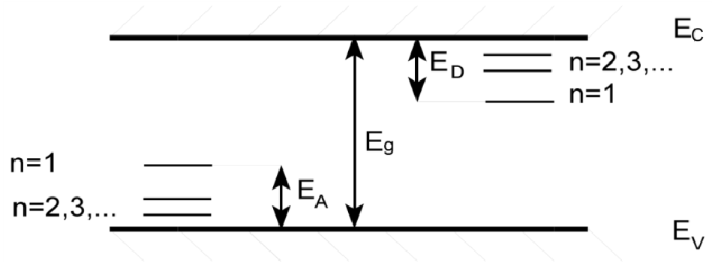
\includegraphics[width=0.55\linewidth]{figures/Energieschme_Halbleiter.png}
    \caption{Schematisches Bändermodell eines Halbleiters mit Valenzband, Leitungsband und verbotener Zone, nach \cite[S.~5--8]{manual}.}
    \label{fig:bandmodell}
\end{figure}

Bei einer strahlenden Band-Band-Rekombination geht ein Elektron aus dem Leitungsband in einen freien Zustand des Valenzbandes über. Die dabei frei werdende Energie kann als Photon emittiert werden. Zwischen Photonenenergie und Wellenlänge gilt
\begin{equation}
    E = h\nu = \frac{hc}{\lambda}.
    \label{eq:photonenergie}
\end{equation}
Damit entspricht eine kurze Emissionswellenlänge einer großen Übergangsenergie.

Wichtig ist außerdem die Unterscheidung zwischen direkten und indirekten Halbleitern. Bei einem direkten Halbleiter liegen Leitungsbandminimum und Valenzbandmaximum beim gleichen Wellenzahlvektor. Die Rekombination kann daher ohne zusätzliche Impulsübertragung erfolgen. Bei einem indirekten Halbleiter liegen diese Extremstellen bei verschiedenen Wellenzahlvektoren. Für einen optischen Übergang muss dann zusätzlich ein Phonon oder eine lokalisierte Störstelle beteiligt sein, um die Impulserhaltung zu erfüllen. Deshalb sind direkte Halbleiter wie GaAs in der Regel effizientere Lichtemitter als indirekte Halbleiter wie GaP \cite[S.~7--8]{manual}.

\subsection{Störstellen und Exzitonen}

Reale Halbleiter enthalten Gitterfehler und Fremdatome. Diese Störstellen beeinflussen die elektrische Leitfähigkeit und die Lumineszenz entscheidend. Donatoren besitzen gegenüber dem ersetzten Gitteratom ein zusätzliches Valenzelektron und erzeugen ein Energieniveau knapp unterhalb des Leitungsbandes. Akzeptoren besitzen ein Valenzelektron weniger und erzeugen ein Niveau knapp oberhalb des Valenzbandes. Die Ionisierungsenergien wasserstoffähnlicher Donator- und Akzeptorzustände können näherungsweise über effektive Massen und die dielektrische Abschirmung beschrieben werden \cite[S.~8--10]{manual}:
\begin{equation}
    E_D = \frac{m_n}{m}\frac{E_H}{\varepsilon^2},
    \qquad
    E_A = \frac{m_p}{m}\frac{E_H}{\varepsilon^2}.
    \label{eq:ionisierungsenergien}
\end{equation}
Hierbei ist $E_H=\SI{13.6}{\electronvolt}$ die Bindungsenergie des Wasserstoffatoms, $m_n$ und $m_p$ sind die effektiven Massen von Elektronen und Löchern, $m$ ist die freie Elektronenmasse und $\varepsilon$ die statische Dielektrizitätskonstante.

Neben Donatoren und Akzeptoren sind isoelektronische Störstellen für diesen Versuch wichtig. Sie besitzen dieselbe Valenzelektronenzahl wie das ersetzte Atom, verändern aber lokal das Kristallpotential. Dadurch können Elektron-Loch-Paare gebunden werden. Ein solches Elektron-Loch-Paar wird als Exziton bezeichnet. Bei einem freien Exziton sind Elektron und Loch durch Coulomb-Wechselwirkung aneinander gebunden, können sich aber als Paar durch den Kristall bewegen. Wird dieses Paar zusätzlich an eine Störstelle gebunden, liegt ein gebundenes Exziton vor. Dessen Energieniveau liegt tiefer als das Niveau des freien Exzitons; die Rekombination liefert daher Photonenenergien unterhalb der Bandlücke \cite[S.~10--11]{manual}. Für ein an eine isoelektronische Störstelle gebundenes Exziton wird im Versuch die Energiebilanz
\begin{equation}
    h\nu_\mathrm{max}=E_g-E_\mathrm{ex}-E_B
    \label{eq:exzitonbilanz}
\end{equation}
verwendet. Dabei ist $E_\mathrm{ex}$ die Ionisierungsenergie des freien Exzitons und $E_B$ die Bindungsenergie des Exzitons an die Störstelle.

\subsection{Zustandsdichte und Fermi-Verteilungsfunktion}

Für die Linienform eines Lumineszenzspektrums ist nicht nur die Lage der Bandkanten relevant, sondern auch die Zahl der verfügbaren Zustände und deren Besetzung. Die Zustandsdichte $\rho(E)$ gibt an, wie viele Zustände pro Energieintervall und Volumeneinheit zur Verfügung stehen. Für parabolische Bänder nimmt die Zustandsdichte mit der Wurzel der Energie relativ zur Bandkante zu \cite[S.~11--12]{manual}. Die Besetzung dieser Zustände wird durch die Fermi-Verteilungsfunktion beschrieben \cite{grundmann2006}:
\begin{equation}
    f(E,T)=\frac{1}{1+\exp\left(\frac{E-E_F}{k_B T}\right)}.
    \label{eq:fermi}
\end{equation}
Bei $T=\SI{0}{\kelvin}$ sind alle Zustände unterhalb des Ferminiveaus $E_F$ besetzt und alle Zustände oberhalb davon unbesetzt. Bei endlicher Temperatur wird dieser Übergang über einen Energiebereich der Größenordnung $k_BT$ verbreitert \cite[S.~12--14]{manual}.

\begin{figure}[H]
    \centering
    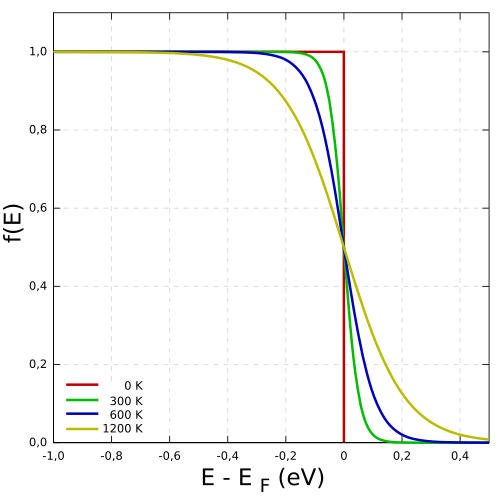
\includegraphics[width=0.48\linewidth]{figures/fermi_verteilung_temperatur.png}
    \caption{Temperaturabhängigkeit der Fermi-Verteilung. Bei höheren Temperaturen wird der Übergang um das Ferminiveau verbreitert, vgl. \cite[S.~12--13]{manual}.}
    \label{fig:fermi}
\end{figure}

Für die Auswertung der $Ga_{1-x}Al_xAs$-Spektren ist diese Überlegung wichtig, weil die Raumtemperatur-Linienform einer Band-Band-Rekombination durch die sogenannte Eagles-Verteilung beschrieben werden kann. Ihr Maximum liegt bei
\begin{equation}
    h\nu_\mathrm{max}=E_g+\frac{k_BT}{2}.
    \label{eq:eaglesmax}
\end{equation}
Aus dem gemessenen Maximum kann daher die Bandlücke des Mischkristalls abgeschätzt werden \cite[S.~24]{manual}.

\subsection{p-n-Übergang}

Ein p-n-Übergang entsteht, wenn ein p-dotierter und ein n-dotierter Bereich aneinandergrenzen. Im thermodynamischen Gleichgewicht diffundieren Elektronen und Löcher über die Grenzfläche und hinterlassen ortsfeste ionisierte Störstellen. Dadurch bildet sich eine Raumladungszone mit einer Diffusionsspannung aus. Im Bändermodell zeigt sich dies als Bandverbiegung \cite[S.~14--15]{manual}.

\begin{figure}[H]
    \centering
    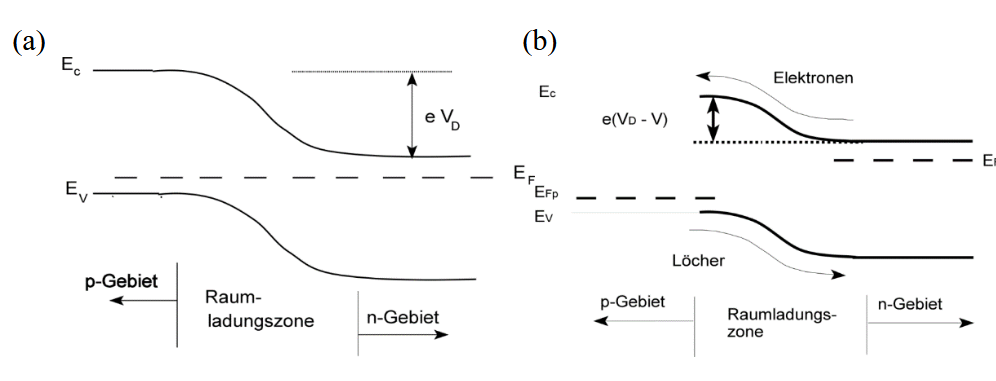
\includegraphics[width=0.58\linewidth]{figures/p-n-ubergang.png}
    \caption{Schematischer p-n-Übergang im Gleichgewicht und in Durchlassrichtung, nach \cite[Abb.~6]{manual}.}
    \label{fig:pn}
\end{figure}

Wird der Übergang in Sperrrichtung gepolt, werden freie Ladungsträger aus der Raumladungszone abgesaugt und der Widerstand steigt. In Durchlassrichtung wird die Potentialbarriere reduziert. Elektronen werden in das p-Gebiet und Löcher in das n-Gebiet injiziert. Diese injizierten Ladungsträger können anschließend rekombinieren. Erfolgt die Rekombination strahlend, entsteht Elektrolumineszenz. Im stationären Betrieb liegt kein thermodynamisches Gleichgewicht mehr vor; stattdessen werden getrennte Quasi-Ferminiveaus für Elektronen und Löcher verwendet \cite[S.~15]{manual}.

\subsection{Rekombinationsmechanismen}

Die im Versuch beobachteten Spektren entstehen durch unterschiedliche Rekombinationsmechanismen. Bei der Band-Band-Rekombination rekombiniert ein Elektron direkt aus dem Leitungsband mit einem Loch im Valenzband. Bei Störstellen-Band-Rekombinationen ist entweder ein Donator- oder ein Akzeptorniveau beteiligt. Zusätzlich kann ein Elektron an einem Donator und ein Loch an einem Akzeptor gebunden sein; die anschließende Donator-Akzeptor-Paarrekombination besitzt näherungsweise die Energie \cite[S.~16--17]{manual}
\begin{equation}
    h\nu = E_g - E_D - E_A + E_C.
    \label{eq:dap}
\end{equation}
Der Coulombterm $E_C$ hängt vom Abstand zwischen Donator und Akzeptor ab. Wird er vernachlässigt, kann aus der Differenz zwischen Bandlücke und Photonenenergie die Summe $E_D+E_A$ abgeschätzt werden.

\begin{figure}[H]
    \centering
    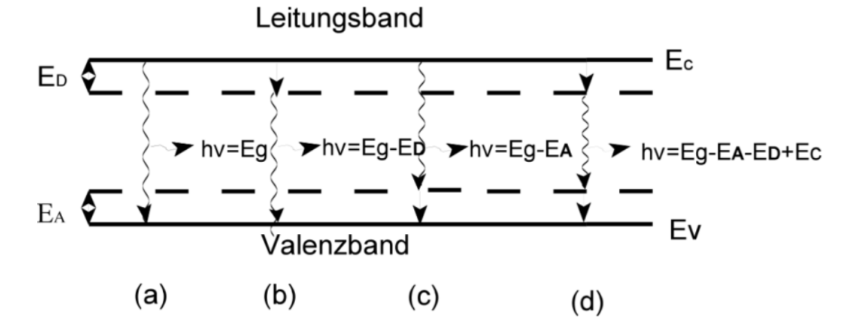
\includegraphics[width=0.58\linewidth]{figures/Rekombinationsmechnismen.png}
    \caption[Rekombinationsmechanismen im Halbleiter]{Schematische Rekombinationsmöglichkeiten im Halbleiter: Band-Band-, Störstellen-Band- und Donator-Akzeptor-Paarrekombination, nach \cite[Abb.~7]{manual}.}
    \label{fig:rekombination}
\end{figure}

Bei indirekten Halbleitern oder bei stark lokalisierten Störstellenzuständen können außerdem Phononen beteiligt sein. Eine Phononenwiederholung erscheint im Spektrum als weiterer Peak oder als Schulter bei niedrigerer Photonenenergie. Im Manual wird für GaP und $Ga_{1-x}Al_xAs$ ein typischer Abstand von einigen zehn Milli-Elektronenvolt diskutiert \cite[S.~22, S.~26]{manual}.

\subsection{Materialien und erwartete Rekombinationen}

\paragraph{GaAs-Diode}
GaAs ist ein direkter Halbleiter und eignet sich daher gut für effiziente Lumineszenzdioden. Bei Raumtemperatur liegt die Bandlücke im nahen Infrarot. Für GaAs wird die temperaturabhängige direkte Bandlücke im Manual durch \cite[S.~19]{manual}
\begin{equation}
    E_{g,d}(GaAs,T)=1.519-\frac{5.404\cdot10^{-4}T^2}{T+204}
    \label{eq:eg_gaas}
\end{equation}
beschrieben, wobei $T$ in Kelvin und $E_g$ in Elektronenvolt einzusetzen sind. Bei Si-dotierten GaAs-Dioden kann Silizium amphoter wirken, also sowohl Donator- als auch Akzeptorzustände erzeugen. Dadurch sind Donator-Akzeptor-Übergänge möglich, deren Photonenenergie unterhalb der ungestörten Bandlücke liegt \cite[S.~17--19]{manual}.

\paragraph{Rotstrahlende Diode Ga(As,P)}
Für rote Lumineszenz wird ein Mischkristall $GaAs_{1-x}P_x$ verwendet. Mit zunehmendem Phosphoranteil $x$ steigt die Bandlücke. Der direkte und der indirekte Übergang schneiden sich bei $x_s$; für $x<x_s$ bleibt der Mischkristall direkt und besitzt eine hohe Übergangswahrscheinlichkeit \cite[S.~19--20]{manual}. Für die Zusammensetzungsabhängigkeit gilt bei \SI{300}{\kelvin}
\begin{align}
    E_{g,d}(x)&=E_{g,d}(0)+[E_{g,d}(1)-E_{g,d}(0)-0.23]x+0.23x^2,
    \label{eq:gaasp_direct}\\
    E_{g,i}(x)&=E_{g,i}(0)+[E_{g,i}(1)-E_{g,i}(0)-0.23]x+0.23x^2.
    \label{eq:gaasp_indirect}
\end{align}
Die Rekombination der roten Diode wird als Übergang vom Leitungsband zu einem Akzeptorniveau beschrieben, sodass $h\nu_\mathrm{max}=E_{g,d}(x)-E_A$ gilt \cite[S.~20]{manual}.

\paragraph{Orangestrahlende Diode Ga(As,P)}
Die orange Diode besteht ebenfalls aus $GaAs_{1-x}P_x$, besitzt aber einen deutlich höheren Phosphoranteil von etwa $x=0.87$. Da dieser Wert oberhalb von $x_s$ liegt, handelt es sich um einen indirekten Halbleiter. Die Emission wird durch Stickstoff als isoelektronische Störstelle ermöglicht. An dieser Störstelle kann ein Exziton gebunden werden, das anschließend strahlend rekombiniert. Die Bindungsenergie $E_B$ wird mit Gleichung~\eqref{eq:exzitonbilanz} abgeschätzt \cite[S.~21]{manual}.

\paragraph{Grünstrahlende Diode GaP}
Die grüne Diode basiert auf stickstoffdotiertem GaP. GaP besitzt bei Raumtemperatur eine indirekte Bandlücke von etwa \SI{2.272}{\electronvolt}. Die Stickstoffstörstellen lokalisieren gebundene Exzitonen und erhöhen dadurch die Wahrscheinlichkeit strahlender Übergänge. Bei hoher Stickstoffkonzentration und Raumtemperatur sind einzelne Linien nicht mehr aufgelöst; stattdessen wird eine breite Lumineszenzbande beobachtet \cite[S.~22--23]{manual}.

\paragraph{Blaustrahlende Diode SiC}
Für blaue Emission werden Materialien mit Bandlücken oberhalb von etwa \SI{2.5}{\electronvolt} benötigt. Im Versuch wird eine SiC-Diode verwendet. SiC kann in mehreren Kristallstrukturen auftreten, deren Bandlücken indirekt sind. Die p- und n-Leitung wird durch Dotierung hergestellt; der genaue Rekombinationsmechanismus wird im Manual nicht weiter festgelegt \cite[S.~23]{manual}.

\paragraph{Photolumineszenz von $Ga_{1-x}Al_xAs$}
Das Mischsystem $Ga_{1-x}Al_xAs$ ist gitterangepasst auf GaAs-Substraten realisierbar. Für $x<0.43$ ist der relevante Übergang direkt und die Bandlücke kann näherungsweise als
\begin{equation}
    E_{g,d}(x,T)=E_{g,d}(GaAs,T)+1.42x
    \label{eq:gaalas}
\end{equation}
geschrieben werden \cite[S.~23--26, Tabelle~2]{manual}. Die Materialparameter für $Ga_{1-x}Al_xAs$ sind im Manual auf Grundlage der Literatur zu Aluminium-Gallium-Arsenid zusammengestellt \cite{adachi1993}. Bei Raumtemperatur dominiert die Band-Band-Rekombination, deren Maximum nach Gleichung~\eqref{eq:eaglesmax} oberhalb der Bandlücke liegt. Bei der Temperatur flüssigen Stickstoffs werden exzitonische Emissionen im Allgemeinen nicht mehr deutlich beobachtet; stattdessen treten Donator-Akzeptor-Paarübergänge und mögliche Phononenwiederholungen auf \cite[S.~24--26]{manual}.

\begin{figure}[H]
    \centering
    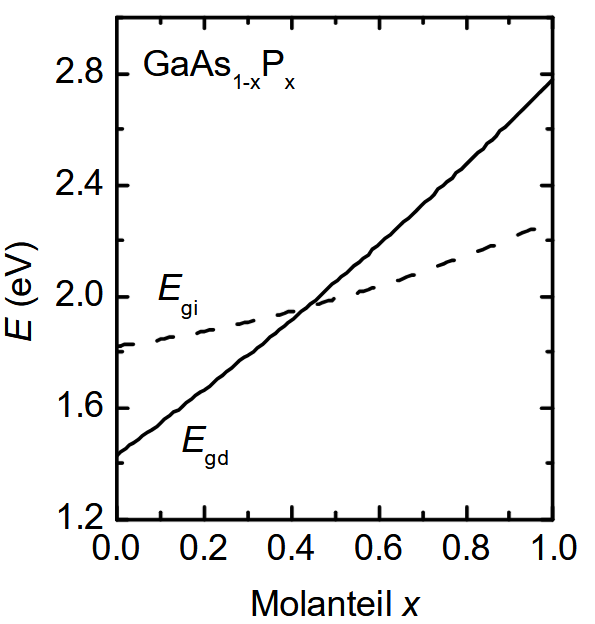
\includegraphics[width=0.60\linewidth]{figures/bandabstaende_gaasp.png}
    \caption{Abhängigkeit der direkten und indirekten Bandabstände vom Molanteil im Mischkristall, nach \cite[Abb.~9]{manual}.}
    \label{fig:bandabstaende}
\end{figure}

\section{Versuchsaufbau}

Der Versuch dient dazu, Lumineszenzspektren als Funktion der Wellenlänge aufzunehmen. Die grundlegende Anordnung besteht aus Lichtquelle beziehungsweise Probe, optischer Abbildung, Chopper, Gittermonochromator, Sekundärelektronenvervielfacher (SEV), Lock-In-Verstärker und Computersteuerung. Die zu untersuchenden Lumineszenzdioden sowie die Natriumdampflampe werden vor dem Kryostat positioniert und bei Raumtemperatur gemessen. Die $Ga_{1-x}Al_xAs$-Proben befinden sich dagegen auf dem Probenhalter des Kryostats und können mit flüssigem Stickstoff gekühlt werden \cite[S.~26--27]{manual}.

\begin{figure}[H]
    \centering
    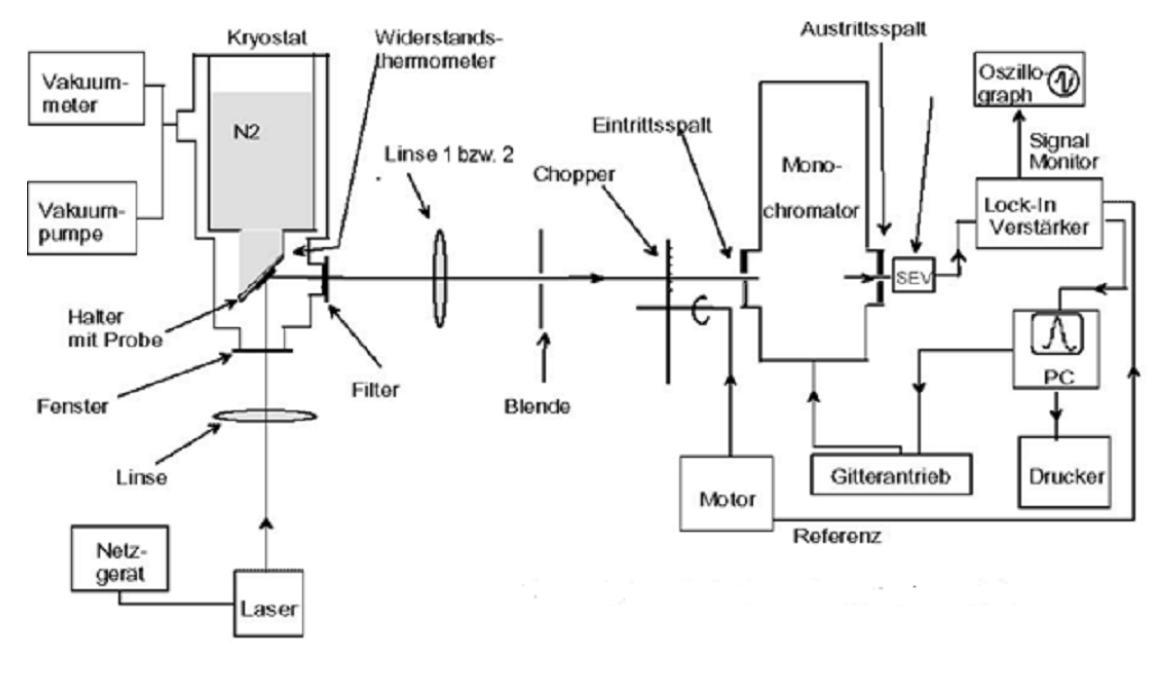
\includegraphics[width=0.85\linewidth]{figures/experimenteller_aufbau.png}
    \caption{Schematischer Messplatz für Photo- und Elektrolumineszenz, nach \cite[Abb.~12]{manual}.}
    \label{fig:aufbau}
\end{figure}

\subsection{Gittermonochromator SP-2155}

Die emittierte Strahlung gelangt über eine Quarzlinse, eine Blende und den Chopper zum Eintrittsspalt des Gittermonochromators SP-2155. Im Monochromator wird das Licht über Spiegel auf ein Reflexionsgitter geführt, dort spektral zerlegt und anschließend am Austrittsspalt wellenlängenselektiv ausgekoppelt. Die Einstellung der Wellenlänge erfolgt über einen computergesteuerten Schrittmotor. Das verwendete Gitter besitzt \SI{1200}{Furchen\per\milli\meter}. Für eine Spaltbreite von \SI{10}{\micro\meter} beträgt die spektrale Breite etwa \SI{0.1}{\nano\meter}; sie skaliert näherungsweise proportional mit der Spaltbreite \cite[S.~30--32]{manual}.

\begin{figure}[H]
    \centering
    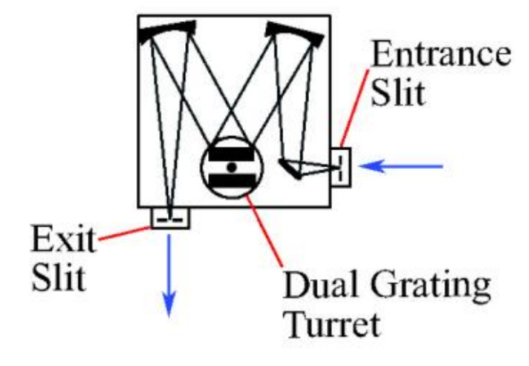
\includegraphics[width=0.82\linewidth]{figures/Gittermonochromator.png}
    \caption{Strahlengang im Gittermonochromator SP-2155, nach \cite[Abb.~16]{manual}.}
    \label{fig:monochromator}
\end{figure}

Hinter dem Monochromator trifft das monochromatische Licht auf den SEV. Der SEV wandelt das Lichtsignal in einen elektrischen Strom um, der anschließend lock-in-verstärkt wird. Da der Chopper das optische Signal periodisch moduliert, kann der Lock-In-Verstärker phasenempfindlich auf diese Modulationsfrequenz messen. Dadurch wird Untergrundlicht stark unterdrückt. Die Ausgangsspannung des Lock-In-Verstärkers ist im verwendeten Bereich proportional zur optischen Signalstärke und wird über einen Analog-Digital-Wandler vom Computer registriert \cite[S.~32--34]{manual}.

\begin{figure}[H]
    \centering
    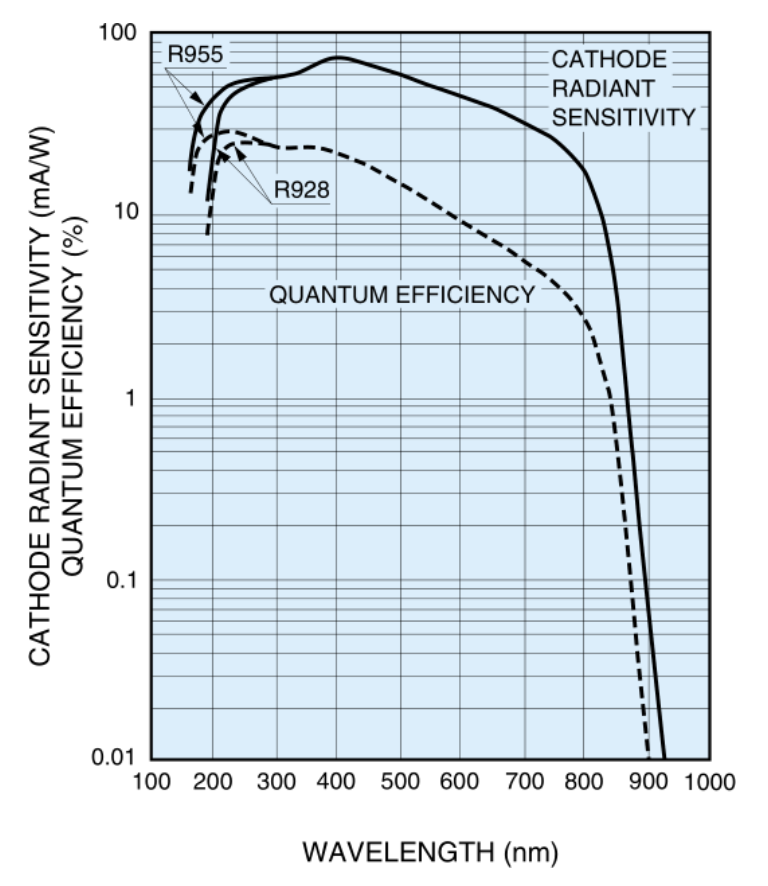
\includegraphics[width=0.75\linewidth]{figures/quantenausbeute.png}
    \caption{Quantenausbeute der im Versuch verwendeten SEV-Typen. Im nahen Infrarot fällt die Empfindlichkeit stark ab, nach \cite[Abb.~19]{manual}.}
    \label{fig:quantenausbeute}
\end{figure}

\subsection{Probenanordnung im Kryostat}

Für die Photolumineszenzmessungen werden die $Ga_{1-x}Al_xAs$-Proben mit einem frequenzverdoppelten Nd:YAG-Laser bei \SI{532}{\nano\meter} angeregt. Der Kryostat wird evakuiert, um den Wärmeaustausch mit der Umgebung zu reduzieren. Die Probe wird über einen Kupferfinger mit flüssigem Stickstoff gekühlt, während die Temperatur in Probennähe mit einem Platin-Widerstandsthermometer bestimmt wird \cite[S.~27--29]{manual}.

\begin{figure}[H]
    \centering
    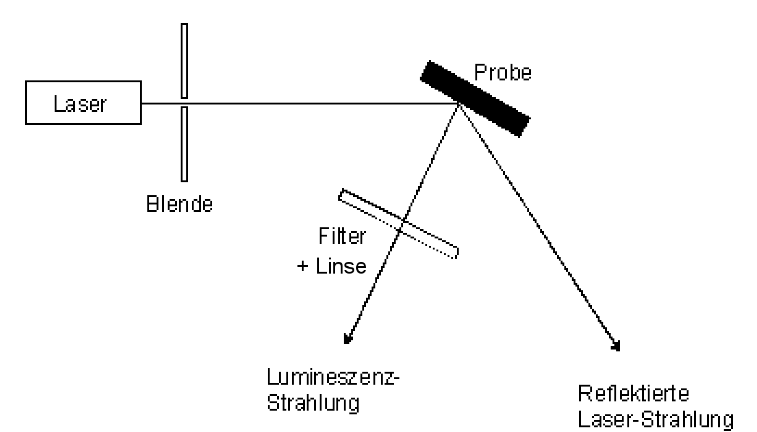
\includegraphics[width=0.65\linewidth]{figures/Probenanordnung_im_Kryostat.png}
    \caption{Probenanordnung im Kryostat. Die Geometrie reduziert den direkten Einfall reflektierter Laserstrahlung in den Monochromator, nach \cite[Abb.~14]{manual}.}
    \label{fig:kryostat_probe}
\end{figure}

Die Probe wird so ausgerichtet, dass reflektierte Laserstrahlung nicht direkt in den Eintrittsspalt des Monochromators fällt. Zusätzlich verhindert ein Kantenfilter, dass Streulicht des Lasers die Messung im Spektralbereich der Photolumineszenz überlagert. Bei sehr intensiven Lichtquellen wie der Natriumdampflampe und der weißen LED wird eine Höhenblende verwendet, um den SEV vor Überlastung zu schützen \cite[S.~29]{manual}.

\section{Auswertung}

Die gemessene Intensität wurde in allen Spektren über die Ausgangsspannung des Detektors dargestellt. Da diese Spannung im verwendeten Arbeitsbereich proportional zur auf den Detektor fallenden Lichtleistung ist, wird sie als relatives Maß für die spektrale Intensität verwendet. Für die Interpretation sind deshalb vor allem die Lage der Maxima, die qualitative Linienform und relative Breiten relevant. Absolute Intensitätsvergleiche zwischen unterschiedlichen Messreihen sind wegen verschiedener Spaltbreiten, Empfindlichkeitseinstellungen und Detektorempfindlichkeiten nur eingeschränkt aussagekräftig.

\subsection{Überprüfung der Eichung der Wellenlängenskala}

\begin{figure}[H]
    \centering
    
\includegraphics[width=1\linewidth]{figures/plot_aufgabe_1.pdf}
    \caption{Eichung der Wellenlängenskala mit Hilfe einer Natriumdampflampe.}
    \label{fig:aufgabe_1}
\end{figure}

\begin{table}[H]
\centering
\caption[Messwerte der Natriumlinien]{Messwerte der 497er-, 589er- und 819er-Linien im Vergleich mit Literaturwerten aus \cite{nist_sodium_2008}. Die Abweichung ist definiert als $\Delta\lambda=\lambda_\mathrm{Lit}-\lambda_\mathrm{Exp}$.}
\label{tab:tabelle_a1}
\begin{tabular}{
  c
  S[table-format=3.2]
  S[table-format=3.2]
  S[table-format=+1.2]
  S[table-format=1.3]
}
\toprule
\textbf{Linie} &
{\textbf{$\lambda_\mathrm{Exp}$ [\si{\nano\meter}]}} &
{\textbf{$\lambda_\mathrm{Lit}$ [\si{\nano\meter}]}} &
{\textbf{$\Delta\lambda$ [\si{\nano\meter}]}} &
{\textbf{FWHM [\si{\nano\meter}]}} \\
\midrule
\multirow{2}{*}{497}
& 498.14 & 498.28 & +0.14 & 0.143 \\
& 497.72 & 497.85 & +0.13 & 0.146 \\
\addlinespace
\multirow{2}{*}{589}
& 589.54 & 589.59 & +0.05 & 0.104 \\
& 588.91 & 589.00 & +0.09 & 0.111 \\
\addlinespace
\multirow{2}{*}{819}
& 819.45 & 819.48 & +0.03 & 0.154 \\
& 818.28 & 818.33 & +0.05 & 0.141 \\
\bottomrule
\end{tabular}
\end{table}

Die in Abbildung~\ref{fig:aufgabe_1} dargestellten Natriumlinien zeigen jeweils zwei Maxima. Dies entspricht der Feinstruktur beziehungsweise Dublettstruktur der ausgewählten Natriumübergänge. Besonders bekannt ist das gelbe Natrium-D-Dublett bei etwa \SI{589}{\nano\meter}; auch im Bereich der 497er- und 819er-Linien treten nahe beieinanderliegende Übergänge auf.

Die experimentell bestimmten Linienpositionen stimmen gut mit den Literaturwerten überein. Die Abweichungen liegen zwischen \SI{0.03}{\nano\meter} und \SI{0.14}{\nano\meter}. Damit ist die Kalibrierung der Wellenlängenskala für die folgenden Messungen ausreichend genau. Ein kleiner systematischer Versatz kann nicht vollständig ausgeschlossen werden, ist jedoch gegenüber den spektralen Breiten der später untersuchten LED- und Photolumineszenzbanden klein.

Die gemessenen Halbwertsbreiten liegen zwischen \SI{0.104}{\nano\meter} und \SI{0.154}{\nano\meter}. Bei einer Spaltbreite von \SI{10}{\micro\meter} beträgt die nominelle spektrale Breite des Monochromators etwa \SI{0.1}{\nano\meter} \cite[S.~32]{manual}. Die gemessenen Werte liegen damit knapp oberhalb der erwarteten instrumentellen Breite. Neben der Monochromatorauflösung tragen endliche Linienbreiten, Justageungenauigkeiten, Rauschen und die Fitmethode zur Halbwertsbreite bei. Für die deutlich breiteren LED-Spektren ist diese Auflösung ausreichend.

\subsection{Spektrum der weiß leuchtenden Diode}

\begin{figure}[H]
    \centering
    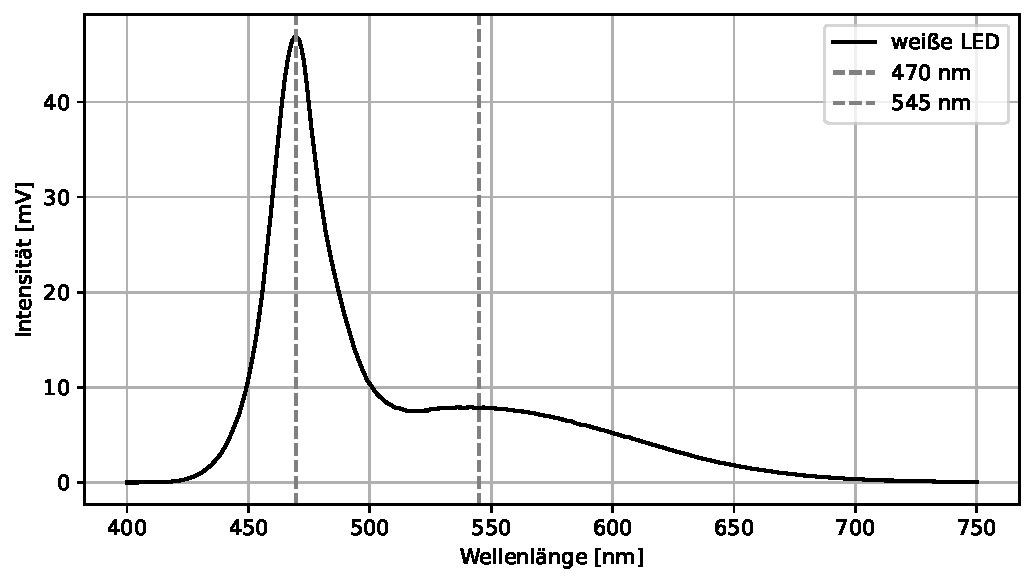
\includegraphics[width=0.75\linewidth]{figures/plot_aufgabe_2.pdf}
    \caption{Spektrum der weiß leuchtenden Diode mit Maxima bei \SI{470.0}{\nano\meter} und \SI{545.0}{\nano\meter}.}
    \label{fig:aufgabe_2}
\end{figure}

Das Spektrum der weiß leuchtenden Diode besitzt zwei deutlich unterscheidbare Beiträge. Das kurzwellige, vergleichsweise schmale Maximum bei \SI{470.0}{\nano\meter} liegt im blauen Spektralbereich. Die zugehörige Photonenenergie beträgt
\begin{equation}
    E_\mathrm{blau}=\frac{\SI{1239.84}{\electronvolt\nano\meter}}{\SI{470.0}{\nano\meter}}
    \approx \SI{2.64}{\electronvolt}.
\end{equation}
Der breitere langwellige Anteil mit einem Maximum bei etwa \SI{545.0}{\nano\meter} entspricht
\begin{equation}
    E_\mathrm{gelb-gruen}\approx
    \frac{\SI{1239.84}{\electronvolt\nano\meter}}{\SI{545.0}{\nano\meter}}
    \approx \SI{2.28}{\electronvolt}.
\end{equation}

Dieses Verhalten ist charakteristisch für eine weiße LED aus blauem Halbleiteremitter und Konversionsschicht. Der blaue Anteil stammt direkt aus der Elektrolumineszenz des Halbleiterchips. Ein Teil dieser Strahlung wird im Leuchtstoff absorbiert und anschließend mit geringerer Photonenenergie wieder emittiert. Die Überlagerung des verbleibenden blauen Lichts mit der breiten gelb-grünen Konversionsbande wird vom Auge als weißes Licht wahrgenommen. Die Breite der Konversionsbande ist daher eine Eigenschaft des Leuchtstoffs und nicht durch die Monochromatorauflösung bestimmt.

\subsection{Spektrum der blau leuchtenden Diode}

\begin{figure}[H]
    \centering
    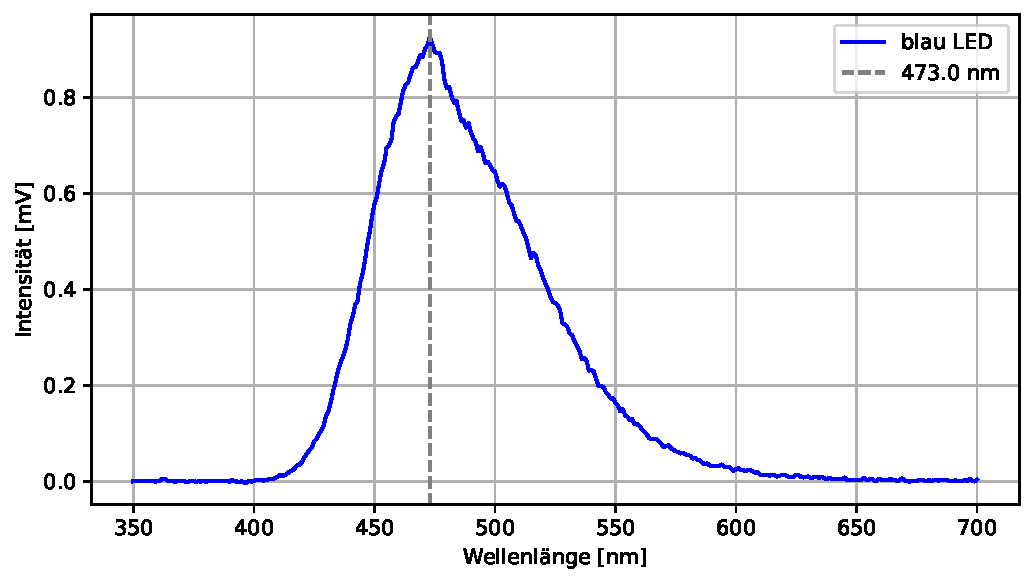
\includegraphics[width=0.75\linewidth]{figures/plot_aufgabe_3.pdf}
    \caption{Spektrum der blau leuchtenden Diode mit einem Maximum bei \SI{473.0}{\nano\meter}.}
    \label{fig:aufgabe_3}
\end{figure}

Die blau leuchtende Diode zeigt ein einzelnes ausgeprägtes Maximum bei \SI{473.0}{\nano\meter}. Die Photonenenergie beträgt
\begin{equation}
    E_\gamma =
    \frac{\SI{1239.84}{\electronvolt\nano\meter}}{\SI{473.0}{\nano\meter}}
    \approx \SI{2.62}{\electronvolt}.
\end{equation}
Diese Energie liegt im Bereich blauer Lumineszenz und stimmt sehr gut mit dem kurzwelligen Maximum der weißen LED überein. Damit wird die Interpretation der weißen LED als Kombination aus blauem Halbleiteremitter und langwelliger Leuchtstoffkonversion gestützt.

Die Emissionsbande ist deutlich breiter als die Kalibrierlinien der Natriumlampe. Bei Raumtemperatur sind die Ladungsträger thermisch verteilt, und die Rekombination erfolgt über energetisch leicht verschiedene Zustände. Zusätzlich verbreitern Materialinhomogenitäten, Dotierungsprofile und Phononenwechselwirkungen das Spektrum.

\subsection{Spektrum der grün leuchtenden Diode}

\begin{figure}[H]
    \centering
    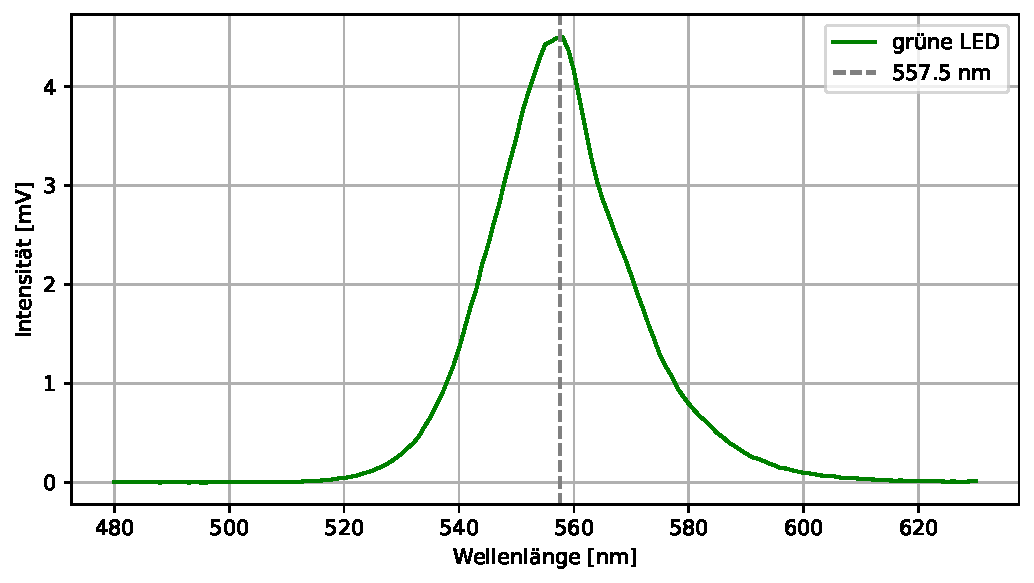
\includegraphics[width=0.75\linewidth]{figures/plot_aufgabe_4.pdf}
    \caption{Spektrum der grün leuchtenden Diode mit einem Maximum bei \SI{557.5}{\nano\meter}.}
    \label{fig:aufgabe_4}
\end{figure}

Das Maximum der grün leuchtenden Diode liegt bei \SI{557.5}{\nano\meter}. Die emittierte Photonenenergie beträgt damit
\begin{equation}
    E_\gamma =
    \frac{\SI{1239.84}{\electronvolt\nano\meter}}{\SI{557.5}{\nano\meter}}
    \approx \SI{2.224}{\electronvolt}.
\end{equation}
Die verwendete grüne Diode basiert auf stickstoffdotiertem GaP. Da GaP ein indirekter Halbleiter ist, wäre eine direkte Band-Band-Rekombination ohne zusätzliche Impulsübertragung nur schwach wahrscheinlich. Die Stickstoffstörstellen wirken jedoch isoelektronisch und lokalisieren gebundene Exzitonen, wodurch strahlende Übergänge wahrscheinlicher werden \cite[S.~22--23]{manual}.

Mit $E_{g,i}(GaP)=\SI{2.272}{\electronvolt}$ und $E_\mathrm{ex}=\SI{0.022}{\electronvolt}$ \cite[Tabelle~3]{manual} ergibt Gleichung~\eqref{eq:exzitonbilanz}
\begin{align}
    E_B &= E_{g,i}-E_\mathrm{ex}-h\nu_\mathrm{max}\\
        &\approx \SI{2.272}{\electronvolt}-\SI{0.022}{\electronvolt}-\SI{2.224}{\electronvolt}\\
        &\approx \SI{0.026}{\electronvolt}.
\end{align}
Die Bindungsenergie des gebundenen Exzitons beträgt somit etwa \SI{26}{\milli\electronvolt}. Der Wert liegt in der erwarteten Größenordnung für gebundene Exzitonen an isoelektronischen Störstellen.

\subsection{Spektrum der orange leuchtenden Diode}

\begin{figure}[H]
    \centering
    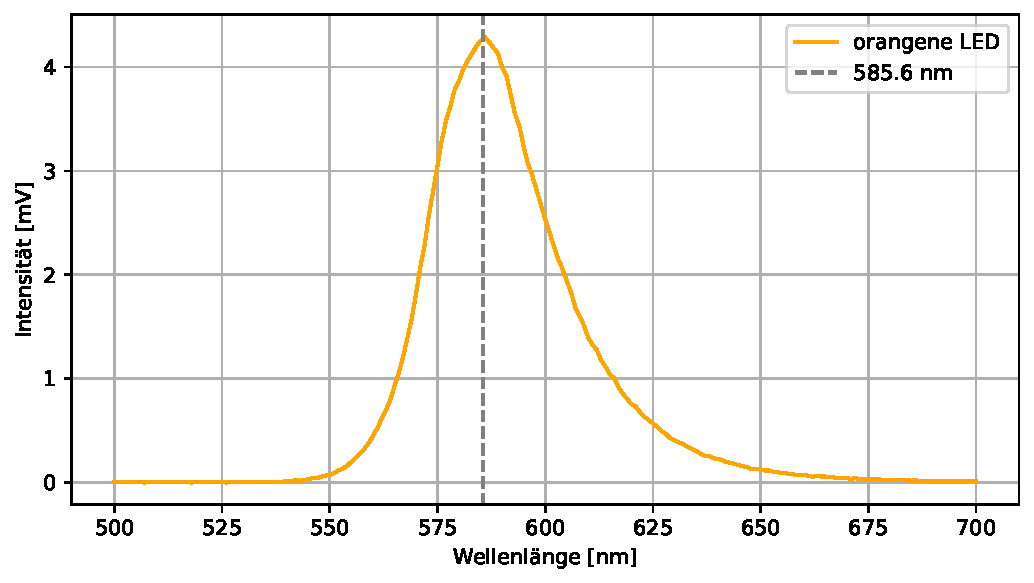
\includegraphics[width=0.75\linewidth]{figures/plot_aufgabe_5.pdf}
    \caption{Spektrum der orange leuchtenden Diode mit einem Maximum bei \SI{585.6}{\nano\meter}.}
    \label{fig:aufgabe_5}
\end{figure}

Die orange leuchtende Diode besitzt ihr Intensitätsmaximum bei \SI{585.6}{\nano\meter}. Daraus folgt
\begin{equation}
    E_\gamma =
    \frac{\SI{1239.84}{\electronvolt\nano\meter}}{\SI{585.6}{\nano\meter}}
    \approx \SI{2.117}{\electronvolt}.
\end{equation}
Für die orange Ga(As,P)-Diode wird ein Phosphoranteil von $x=0.87$ verwendet \cite[S.~21]{manual}. Die indirekte Bandlücke des Mischkristalls ergibt sich aus Gleichung~\eqref{eq:gaasp_indirect} mit $E_{g,i}(0)=\SI{1.82}{\electronvolt}$ und $E_{g,i}(1)=\SI{2.272}{\electronvolt}$ zu
\begin{align}
    E_{g,i}(0.87)
    &= \SI{1.82}{\electronvolt}
    +(\SI{2.272}{\electronvolt}-\SI{1.82}{\electronvolt}-\SI{0.23}{\electronvolt})\cdot0.87
    +\SI{0.23}{\electronvolt}\cdot0.87^2\\
    &\approx \SI{2.187}{\electronvolt}.
\end{align}
Mit $E_\mathrm{ex}=\SI{0.022}{\electronvolt}$ folgt
\begin{align}
    E_B &= E_{g,i}(0.87)-E_\mathrm{ex}-h\nu_\mathrm{max}\\
        &\approx \SI{2.187}{\electronvolt}-\SI{0.022}{\electronvolt}-\SI{2.117}{\electronvolt}\\
        &\approx \SI{0.048}{\electronvolt}.
\end{align}
Die Bindungsenergie des gebundenen Exzitons beträgt damit etwa \SI{48}{\milli\electronvolt}. Der größere Wert im Vergleich zur grünen GaP-Diode ist plausibel, da die veränderte Materialzusammensetzung und die Störstellenumgebung die Lokalisierung des Exzitons beeinflussen.

\subsection{Spektrum der rot leuchtenden Diode}

\begin{figure}[H]
    \centering
    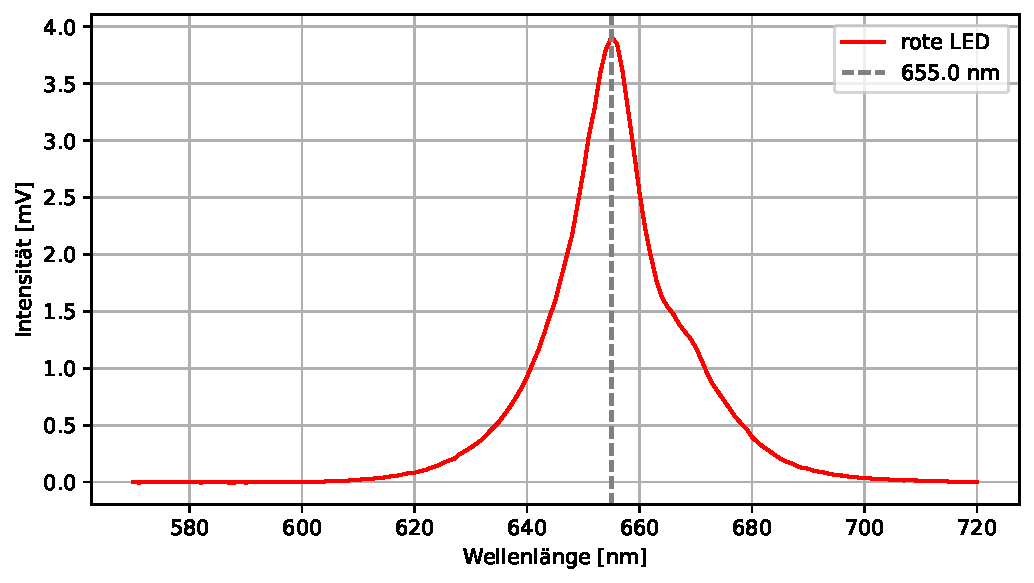
\includegraphics[width=0.75\linewidth]{figures/plot_aufgabe_6.pdf}
    \caption{Spektrum der rot leuchtenden Diode mit einem Maximum bei \SI{655.0}{\nano\meter}.}
    \label{fig:aufgabe_6}
\end{figure}

Das Spektrum der roten Diode zeigt ein Maximum bei \SI{655.0}{\nano\meter}. Die zugehörige Photonenenergie ist
\begin{equation}
    h\nu_\mathrm{max}=
    \frac{\SI{1239.84}{\electronvolt\nano\meter}}{\SI{655.0}{\nano\meter}}
    \approx \SI{1.893}{\electronvolt}.
\end{equation}
Für die rote Ga(As,P)-Diode wird die Emission als Übergang vom Leitungsband zu einem Akzeptorniveau betrachtet \cite[S.~20]{manual}. In guter Näherung wird für die Akzeptorenergie der GaAs-Wert verwendet. Mit $m_p=0.50m$, $\varepsilon=12.9$ und $E_H=\SI{13.6}{\electronvolt}$ \cite[Tabelle~2]{manual} folgt
\begin{equation}
    E_A = \frac{0.50\cdot\SI{13.6}{\electronvolt}}{12.9^2}
    \approx \SI{0.0409}{\electronvolt}.
\end{equation}
Somit ergibt sich für die direkte Bandlücke des Mischkristalls
\begin{equation}
    E_{g,d}(x)=h\nu_\mathrm{max}+E_A
    \approx \SI{1.893}{\electronvolt}+\SI{0.0409}{\electronvolt}
    \approx \SI{1.934}{\electronvolt}.
\end{equation}

Einsetzen in die Gleichung für den direkten Übergang~\eqref{eq:gaasp_direct} mit $E_{g,d}(0)=\SI{1.43}{\electronvolt}$ und $E_{g,d}(1)=\SI{2.781}{\electronvolt}$ ergibt
\begin{equation}
    1.934 = 1.43 + (2.781-1.43-0.23)x+0.23x^2.
\end{equation}
Die physikalisch sinnvolle Lösung der quadratischen Gleichung ist
\begin{equation}
    x \approx 0.414.
\end{equation}
Der Phosphoranteil beträgt damit etwa \SI{41.4}{\percent}; der Arsengehalt ist entsprechend
\begin{equation}
    1-x \approx 0.586,
\end{equation}
also etwa \SI{58.6}{\percent}.

Der Übergang zwischen direktem und indirektem Verhalten ergibt sich aus dem Schnittpunkt von $E_{g,d}(x)$ und $E_{g,i}(x)$. Mit den Parametern aus dem Manual folgt
\begin{equation}
    x_s \approx 0.434.
\end{equation}
Da $x\approx0.414<x_s$ gilt, befindet sich der Mischkristall noch im direkten Bereich. Dies erklärt die vergleichsweise intensive rote Elektrolumineszenz.

\subsection{Spektrum der Infrarot emittierenden GaAs-Diode}

\begin{figure}[H]
    \centering
    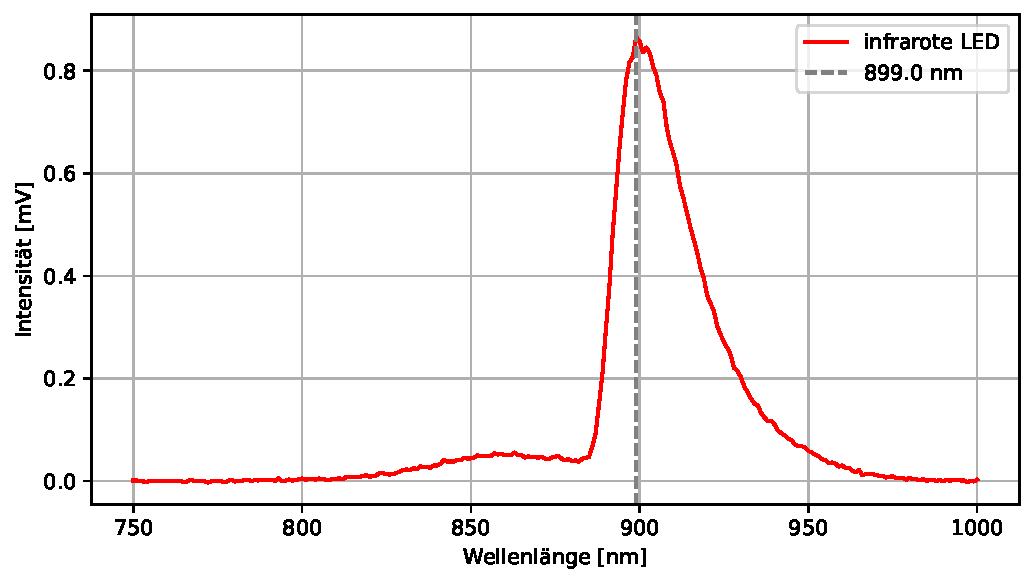
\includegraphics[width=0.75\linewidth]{figures/plot_aufgabe_7.pdf}
    \caption{Spektrum der Infrarot emittierenden GaAs-Diode mit einem Maximum bei \SI{899.0}{\nano\meter}.}
    \label{fig:aufgabe_7}
\end{figure}

\begin{figure}[H]
    \centering
    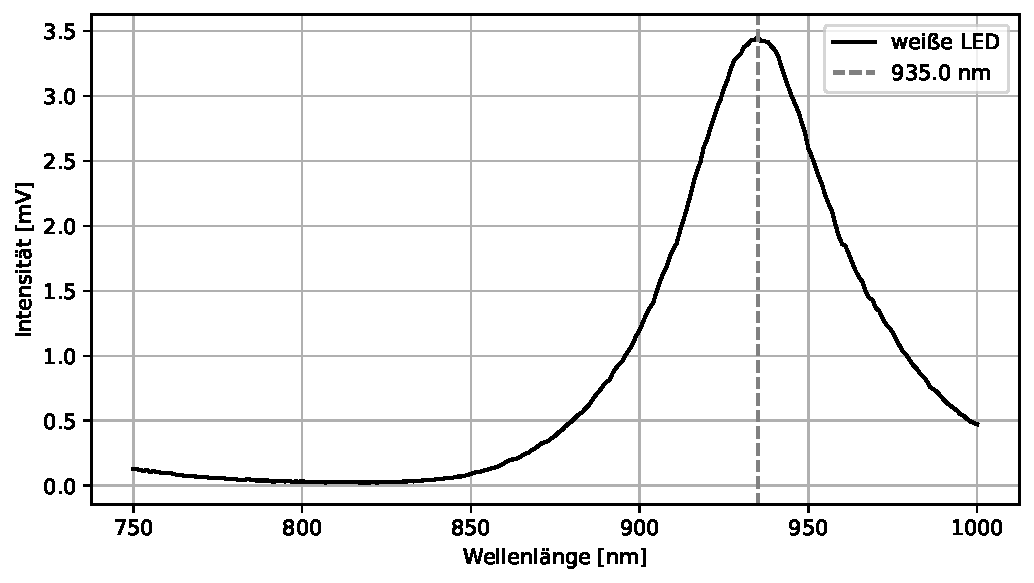
\includegraphics[width=0.75\linewidth]{figures/plot_aufgabe_7alternative.pdf}
    \caption{Optional gemessenes Infrarotspektrum der weißen LED mit einem Maximum bei \SI{935.0}{\nano\meter}.}
    \label{fig:aufgabe_7alternative}
\end{figure}

Das Maximum der GaAs-Diode liegt bei \SI{899.0}{\nano\meter}. Die zugehörige Photonenenergie beträgt
\begin{equation}
    E_\mathrm{exp}=
    \frac{\SI{1239.84}{\electronvolt\nano\meter}}{\SI{899.0}{\nano\meter}}
    \approx \SI{1.379}{\electronvolt}.
\end{equation}
Mit Gleichung~\eqref{eq:eg_gaas} ergibt sich für Raumtemperatur $T=\SI{293.15}{\kelvin}$
\begin{equation}
    E_g(GaAs,T)=1.519-\frac{5.404\cdot10^{-4}T^2}{T+204}
    \approx \SI{1.426}{\electronvolt}.
\end{equation}
Die gemessene Photonenenergie liegt somit um etwa
\begin{equation}
    \Delta E=E_g-E_\mathrm{exp}
    \approx \SI{1.426}{\electronvolt}-\SI{1.379}{\electronvolt}
    \approx \SI{46}{\milli\electronvolt}
\end{equation}
unterhalb der Bandlücke. Eine reine Band-Band-Rekombination erklärt das Maximum daher nicht vollständig.

Die Differenz ist mit Donator-Akzeptor-Rekombinationen im Si-dotierten GaAs vereinbar. Silizium kann in GaAs amphoter eingebaut werden: Auf einem Ga-Platz wirkt es als Donator, auf einem As-Platz als Akzeptor \cite[S.~18]{manual}. Mit $m_n=0.067m$, $m_p=0.50m$ und $\varepsilon=12.9$ \cite[Tabelle~2]{manual} erhält man
\begin{align}
    E_D &= \frac{0.067\cdot\SI{13.6}{\electronvolt}}{12.9^2}
    \approx \SI{5.48}{\milli\electronvolt},\\
    E_A &= \frac{0.50\cdot\SI{13.6}{\electronvolt}}{12.9^2}
    \approx \SI{40.86}{\milli\electronvolt}.
\end{align}
Für eine Donator-Akzeptor-Rekombination ohne Coulombterm ergibt sich damit
\begin{equation}
    E_g-E_D-E_A
    \approx \SI{1.426}{\electronvolt}-\SI{0.00548}{\electronvolt}-\SI{0.04086}{\electronvolt}
    \approx \SI{1.379}{\electronvolt}.
\end{equation}
Dieser Wert stimmt sehr gut mit der experimentellen Energie des Maximums überein. Das beobachtete Infrarotmaximum ist daher wesentlich durch Störstellenübergänge im dotierten GaAs geprägt.

Der Vergleich mit der SEV-Quantenausbeute in Abbildung~\ref{fig:quantenausbeute} zeigt außerdem, dass die Empfindlichkeit des SEV im nahen Infrarot stark abnimmt. Die gemessenen Spannungen sind daher klein, und die Lage schwacher Maxima ist empfindlicher gegenüber Rauschen, Untergrundabzug und Justage. Das optionale Spektrum der weißen LED bei \SI{935.0}{\nano\meter} dient deshalb nur als qualitativer Vergleich im nahinfraroten Messbereich und wird nicht als GaAs-Bandkantenemission interpretiert.

\subsection{Temperaturabhängigkeit der Photolumineszenz von $Ga_{1-x}Al_xAs$}

\begin{figure}[H]
    \centering
    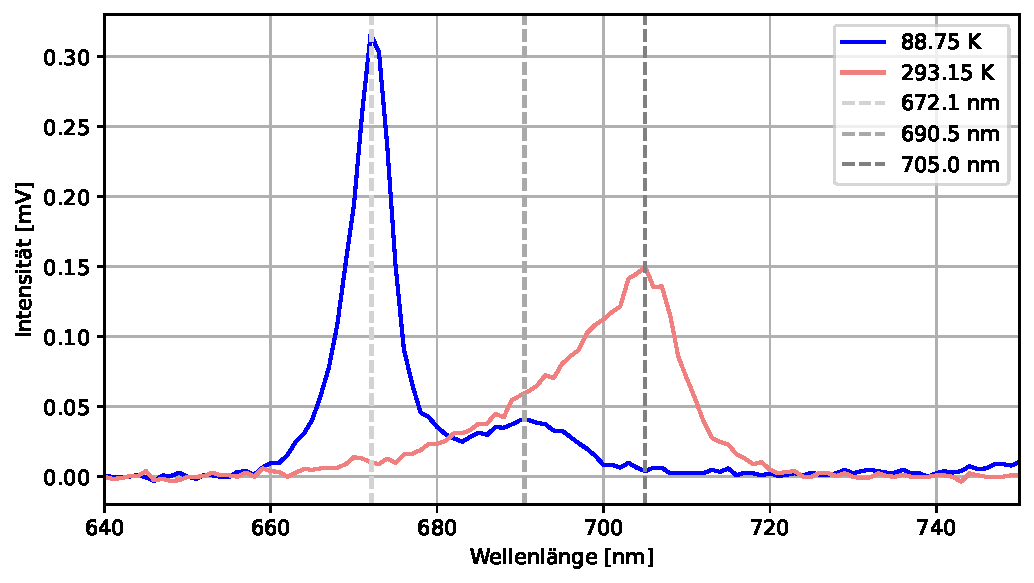
\includegraphics[width=0.75\linewidth]{figures/plot_aufgabe_8_1127.pdf}
    \caption{Spektrum der Probe 1127 bei \SI{293.15}{\kelvin} und \SI{88.75}{\kelvin}. Die Maxima liegen bei \SI{705.0}{\nano\meter} für die warme Messung sowie bei \SI{672.1}{\nano\meter} und \SI{690.5}{\nano\meter} für die kalte Messung.}
    \label{fig:aufgabe_8_1127}
\end{figure}

\begin{figure}[H]
    \centering
    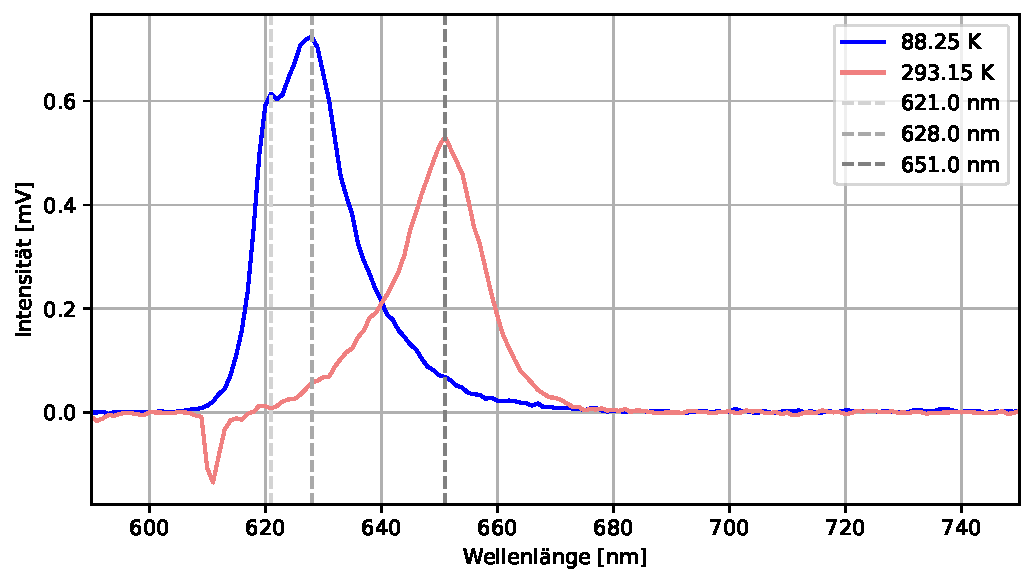
\includegraphics[width=0.75\linewidth]{figures/plot_aufgabe_8_87063.pdf}
    \caption{Spektrum der Probe 87063 bei \SI{293.15}{\kelvin} und \SI{88.25}{\kelvin}. Die Maxima liegen bei \SI{651.0}{\nano\meter} für die warme Messung sowie bei \SI{621.0}{\nano\meter} und \SI{628.0}{\nano\meter} für die kalte Messung.}
    \label{fig:aufgabe_8_87063}
\end{figure}

Zur eindeutigen Zuordnung werden die beiden Messreihen nach den Dateibezeichnungen der Abbildungen als Probe 1127 und Probe 87063 bezeichnet. Beide Proben zeigen beim Abkühlen auf flüssige-Stickstoff-Temperatur eine Verschiebung der Lumineszenz zu kürzeren Wellenlängen. Dies entspricht einer höheren Photonenenergie und ist qualitativ mit der Zunahme der Bandlücke bei sinkender Temperatur vereinbar.

Bei Raumtemperatur wird die Emission näherungsweise als Band-Band-Rekombination beschrieben. Nach der Eagles-Verteilung liegt das Maximum bei $E_g+k_BT/2$ \cite[S.~24]{manual}. Deshalb gilt
\begin{equation}
    E_{g,d}(x,T_\mathrm{warm})
    \approx \frac{hc}{\lambda_\mathrm{warm}}-\frac{k_BT_\mathrm{warm}}{2}.
    \label{eq:x_warm}
\end{equation}
Mit $T_\mathrm{warm}=\SI{293.15}{\kelvin}$ ergibt sich für GaAs
\begin{equation}
    E_{g,d}(GaAs,T_\mathrm{warm})\approx\SI{1.426}{\electronvolt}.
\end{equation}
Der Aluminiumanteil folgt aus Gleichung~\eqref{eq:gaalas}:
\begin{equation}
    x=\frac{E_{g,d}(x,T_\mathrm{warm})-E_{g,d}(GaAs,T_\mathrm{warm})}{1.42}.
\end{equation}

Für Probe 1127 mit $\lambda_\mathrm{warm}=\SI{705.0}{\nano\meter}$ erhält man
\begin{align}
    h\nu_\mathrm{warm} &=
    \frac{\SI{1239.84}{\electronvolt\nano\meter}}{\SI{705.0}{\nano\meter}}
    \approx \SI{1.759}{\electronvolt},\\
    E_{g,d}(x,T_\mathrm{warm}) &\approx
    \SI{1.759}{\electronvolt}-\frac{k_B\cdot\SI{293.15}{\kelvin}}{2}
    \approx \SI{1.746}{\electronvolt},\\
    x_{1127} &\approx
    \frac{\SI{1.746}{\electronvolt}-\SI{1.426}{\electronvolt}}{\SI{1.42}{\electronvolt}}
    \approx 0.226.
\end{align}
Für Probe 87063 mit $\lambda_\mathrm{warm}=\SI{651.0}{\nano\meter}$ folgt analog
\begin{align}
    h\nu_\mathrm{warm} &\approx \SI{1.905}{\electronvolt},\\
    E_{g,d}(x,T_\mathrm{warm}) &\approx \SI{1.892}{\electronvolt},\\
    x_{87063} &\approx 0.328.
\end{align}
Probe 87063 besitzt damit den größeren Aluminiumanteil und entsprechend die größere Bandlücke, was mit ihrer kürzeren Emissionswellenlänge übereinstimmt. Beide Werte liegen unterhalb von $x_s\approx0.43$, sodass die Proben im direkten Bereich des Mischsystems liegen \cite[S.~23--26]{manual}.

Für die kalten Spektren werden die in den Messplots angegebenen Temperaturen verwendet. Damit ist
\begin{align}
    E_{g,d}(GaAs,\SI{88.75}{\kelvin})&\approx\SI{1.504}{\electronvolt},\\
    E_{g,d}(GaAs,\SI{88.25}{\kelvin})&\approx\SI{1.505}{\electronvolt}.
\end{align}
Mit den oben bestimmten Aluminiumanteilen ergeben sich für die kalten Bandkanten
\begin{align}
    E_{g,d}^{1127}(\SI{88.75}{\kelvin})
    &\approx \SI{1.504}{\electronvolt}+1.42\cdot0.226
    \approx \SI{1.825}{\electronvolt},\\
    E_{g,d}^{87063}(\SI{88.25}{\kelvin})
    &\approx \SI{1.505}{\electronvolt}+1.42\cdot0.328
    \approx \SI{1.971}{\electronvolt}.
\end{align}
Wenn ein tieftemperierter Peak als Donator-Akzeptor-Paarübergang interpretiert wird und der Coulombterm aus Gleichung~\eqref{eq:dap} vernachlässigt wird, gilt
\begin{equation}
    E_D+E_A\approx E_g(x,T_\mathrm{kalt})-h\nu_\mathrm{kalt}.
    \label{eq:stoerstellen_abschaetzung}
\end{equation}

Bei Probe 1127 liegt neben dem hochenergetischen Peak bei \SI{672.1}{\nano\meter} eine langwelligere Struktur bei \SI{690.5}{\nano\meter}. Für diese Struktur ergibt sich
\begin{align}
    h\nu(\SI{690.5}{\nano\meter}) &\approx
    \frac{\SI{1239.84}{\electronvolt\nano\meter}}{\SI{690.5}{\nano\meter}}
    \approx \SI{1.796}{\electronvolt},\\
    E_D+E_A &\approx
    \SI{1.825}{\electronvolt}-\SI{1.796}{\electronvolt}
    \approx \SI{29}{\milli\electronvolt}.
\end{align}
Dieser Wert liegt in der Größenordnung der im Manual angegebenen Akzeptorenergien für $Ga_{1-x}Al_xAs$ bei $x\approx0.23$. Beispielsweise ergeben die dort angegebenen Parameter grob \SIrange{28}{38}{\milli\electronvolt} für C-, Mg- oder Zn-Akzeptoren, während Si- und Ge-Akzeptoren höher liegen \cite[Tabelle~2]{manual}. Der Peak bei \SI{672.1}{\nano\meter} liegt dagegen um etwa \SI{20}{\milli\electronvolt} oberhalb der so abgeschätzten kalten Bandkante. Er wird deshalb nicht zur Bestimmung einer Störstellenenergie verwendet, sondern als bandkantennaher Peak mit Mess- beziehungsweise Fitunsicherheit oder als nicht vollständig aufgelöste Überlagerung interpretiert. Eine eindeutige Störstellenidentifikation ist insgesamt nicht möglich, weil der Donatorbeitrag, der Coulombterm des Donator-Akzeptor-Paares und mögliche Phononenbeiträge nicht getrennt bestimmt werden.

Bei Probe 87063 liegt der Peak bei \SI{628.0}{\nano\meter} mit
\begin{equation}
    h\nu(\SI{628.0}{\nano\meter})\approx\SI{1.974}{\electronvolt}
\end{equation}
innerhalb weniger Milli-Elektronenvolt an der aus der Raumtemperaturmessung berechneten kalten Bandkante $E_{g,d}^{87063}(\SI{88.25}{\kelvin})\approx\SI{1.971}{\electronvolt}$. Gleichung~\eqref{eq:stoerstellen_abschaetzung} würde formal einen leicht negativen Wert von etwa \SI{-3}{\milli\electronvolt} liefern. Da eine negative Störstellenenergie unphysikalisch ist, wird dieser Peak nicht als Donator-Akzeptor-Paarübergang gewertet, sondern als Bandkantenpeak innerhalb der Unsicherheit der Temperatur- und Peakbestimmung.

Der Peak bei \SI{621.0}{\nano\meter} besitzt mit
\begin{equation}
    h\nu(\SI{621.0}{\nano\meter})\approx\SI{1.997}{\electronvolt}
\end{equation}
eine noch höhere Energie und liegt damit etwa \SI{26}{\milli\electronvolt} oberhalb der abgeschätzten Bandkante. Diese Zuordnung ist für einen einfachen Bandkanten- oder Donator-Akzeptor-Übergang nicht konsistent. Plausibel ist daher, dass es sich um ein Mess- oder Auswerteartefakt, eine Fitunsicherheit durch die überlagerte Schulterstruktur oder um eine fehlerhaft bestimmte Peaklage handelt. Für eine belastbare Störstellenenergie der Probe 87063 sollte der \SI{621}{\nano\meter}-Peak daher nicht verwendet werden.

Insgesamt zeigen die kalten Spektren dennoch klar, dass bei tieferen Temperaturen zusätzliche Strukturen sichtbar werden, die bei Raumtemperatur thermisch verbreitert oder überlagert sind. Die Verschiebung der Hauptmaxima zu kürzeren Wellenlängen bestätigt qualitativ die Vergrößerung der Bandlücke bei sinkender Temperatur.

\section{Zusammenfassung}

Im Versuch wurde zunächst die Wellenlängenskala des Gittermonochromators mit Natriumlinien überprüft. Die gemessenen Linienpositionen wichen nur um \SIrange{0.03}{0.14}{\nano\meter} von den Literaturwerten ab. Die Halbwertsbreiten lagen mit \SIrange{0.104}{0.154}{\nano\meter} knapp oberhalb der nominellen spektralen Breite bei einer Spaltbreite von \SI{10}{\micro\meter}. Der Monochromator war damit für die anschließende Untersuchung der deutlich breiteren Lumineszenzspektren hinreichend kalibriert.

Die weiße LED zeigte ein schmales blaues Maximum bei \SI{470.0}{\nano\meter} und eine breite Konversionsbande bei \SI{545.0}{\nano\meter}. Dies bestätigt das typische Funktionsprinzip einer weißen LED aus blauem Halbleiteremitter und Leuchtstoffschicht. Die separat gemessene blaue Diode besaß ihr Maximum bei \SI{473.0}{\nano\meter} und stützte diese Interpretation.

Für die grüne GaP-Diode wurde aus dem Maximum bei \SI{557.5}{\nano\meter} eine Bindungsenergie des an Stickstoff gebundenen Exzitons von etwa \SI{26}{\milli\electronvolt} bestimmt. Für die orange Ga(As,P)-Diode ergab sich aus dem Maximum bei \SI{585.6}{\nano\meter} eine Exziton-Bindungsenergie von etwa \SI{48}{\milli\electronvolt}. Bei der roten Diode führte das Maximum bei \SI{655.0}{\nano\meter} auf einen Phosphoranteil von ungefähr $x=0.414$ und damit auf einen Arsengehalt von etwa \SI{58.6}{\percent}. Da $x<x_s\approx0.434$ gilt, liegt der Mischkristall noch im direkten Bereich.

Die infrarote GaAs-Diode zeigte ein Maximum bei \SI{899.0}{\nano\meter}, entsprechend \SI{1.379}{\electronvolt}. Dieser Wert liegt um etwa \SI{46}{\milli\electronvolt} unterhalb der GaAs-Bandlücke bei Raumtemperatur und stimmt sehr gut mit der erwarteten Energie einer Donator-Akzeptor-Rekombination unter Beteiligung von Si-Störstellen überein. Die berechneten Ionisierungsenergien betragen $E_D\approx\SI{5.48}{\milli\electronvolt}$ und $E_A\approx\SI{40.86}{\milli\electronvolt}$.

Bei den $Ga_{1-x}Al_xAs$-Proben wurde beim Abkühlen auf flüssige-Stickstoff-Temperatur eine Verschiebung der Lumineszenz zu kürzeren Wellenlängen beobachtet. Dies entspricht der Zunahme der Bandlücke bei sinkender Temperatur. Aus den Raumtemperaturmaxima wurden Aluminiumanteile von etwa $x_{1127}=0.226$ und $x_{87063}=0.328$ abgeschätzt. Für Probe 1127 liefert die langwellige kalte Struktur bei der tatsächlich gemessenen Temperatur von \SI{88.75}{\kelvin} eine Störstellenenergie von etwa \SI{29}{\milli\electronvolt}, was in der Größenordnung typischer Akzeptorenergien liegt. Für Probe 87063 lässt sich aus den kalten Peaks bei \SI{88.25}{\kelvin} keine belastbare positive Störstellenenergie bestimmen: Der Peak bei \SI{628}{\nano\meter} wird als bandkantennah interpretiert, während der Peak bei \SI{621}{\nano\meter} wahrscheinlich auf Artefakt, Fitunsicherheit oder eine fehlerhafte Peakbestimmung zurückgeht.

\newpage
\listoffigures
\listoftables
\printbibliography

\end{document}
